\documentclass{exam}
\usepackage[utf8]{inputenc}
\usepackage{lmodern}
\usepackage{microtype}

% \usepackage[parfill]{parskip}
\usepackage[dvipsnames]{xcolor}
\usepackage{amsmath}
\usepackage{amsfonts}
\usepackage{amsthm}
\usepackage{siunitx}
\DeclareSIUnit\year{yr}
\DeclareSIUnit\foot{ft}
\DeclareSIUnit\litre{\liter}

\usepackage{skull}

\usepackage{pgfplots}
\usepgfplotslibrary{polar}
\pgfplotsset{compat=1.11}
\usepgfplotslibrary{statistics}
\usepackage{graphicx}
\usepackage{sidecap}
\sidecaptionvpos{figure}{c}
\usepackage{float}
\usepackage{gensymb}
\usepackage{tkz-euclide}
\usetkzobj{all}
\usepackage{commath}
\usepackage{hyperref}
\usepackage{enumitem}
\usepackage{wasysym}
\usepackage{multicol}
\usepackage{mathtools}
\usepackage{tcolorbox}
\usepackage{tabularx}
\usepackage[version=4]{mhchem}
\usepackage{changepage}
\usepackage{listings}
\lstset{basicstyle=\ttfamily\linespread{0.8}\small}

\renewcommand*{\thefootnote}{\fnsymbol{footnote}}

\newtheorem*{thm}{Theorem}
\newtheorem*{iden}{Identity}
\newtheorem*{lemma}{Lemma}
\newtheorem{obs}{Observation}
\theoremstyle{definition}
\newtheorem*{defn}{Definition}
\newtheorem*{ex}{Example}
\newtheorem{con}{Construction}
\newtheorem*{alg}{Algorithm}

\newtheoremstyle{break}
  {\topsep}{\topsep}%
  {\itshape}{}%
  {\bfseries}{}%
  {\newline}{}%
\theoremstyle{break}
\newtheorem*{bthm}{Theorem}

% russian integral
\usepackage{scalerel}
\DeclareMathOperator*{\rint}{\scalerel*{\rotatebox{17}{$\!\int\!$}}{\int}}

% \DeclareMathOperator*{\rint}{\int}

\pgfplotsset{vasymptote/.style={
    before end axis/.append code={
        \draw[densely dashed] ({rel axis cs:0,0} -| {axis cs:#1,0})
        -- ({rel axis cs:0,1} -| {axis cs:#1,0});
    }
}}

% \pointsinrightmargin
\boxedpoints
\pointname{}

\newcommand{\questioA}{\question[\texttt{\textbf{\color{Cerulean} A}}]}
\newcommand{\questioM}{\question[\texttt{\textbf{\color{PineGreen} M}}]}
\newcommand{\questioE}{\question[\texttt{\textbf{\color{WildStrawberry} E}}]}
\newcommand{\questioS}{\question[\texttt{\textbf{\color{Goldenrod} S}}]}
\newcommand{\questioO}{\question[\texttt{\textbf{\color{BurntOrange} O}}]}

\newcommand{\parA}{\part[\texttt{\textbf{\color{Cerulean} A}}]}
\newcommand{\parM}{\part[\texttt{\textbf{\color{PineGreen} M}}]}
\newcommand{\parE}{\part[\texttt{\textbf{\color{WildStrawberry} E}}]}
\newcommand{\parS}{\part[\texttt{\textbf{\color{Goldenrod} S}}]}
\newcommand{\parO}{\part[\texttt{\textbf{\color{BurntOrange} O}}]}

\newcommand{\subparA}{\subpart[\texttt{\textbf{\color{Cerulean} A}}]}
\newcommand{\subparM}{\subpart[\texttt{\textbf{\color{PineGreen} M}}]}
\newcommand{\subparE}{\subpart[\texttt{\textbf{\color{WildStrawberry} E}}]}
\newcommand{\subparS}{\subpart[\texttt{\textbf{\color{Goldenrod} S}}]}
\newcommand{\subparO}{\subpart[\texttt{\textbf{\color{BurntOrange} O}}]}

\newcommand{\mainHeader}[2]{\section*{NCEA Level 2 Mathematics\\#1. #2}}
\newcommand{\mainHeaderHw}[2]{\section*{NCEA Level 2 Mathematics (Homework)\\#1. #2}}
\newcommand{\seealso}[1]{\begin{center}\emph{See also #1.}\end{center}}
\newcommand{\drills}[1]{\begin{center}\emph{Drill problems: #1.}\end{center}}
\newcommand{\basedon}[1]{\begin{center}\emph{Notes largely based on #1.}\end{center}}


\begin{document}

\mainHeaderHw{19}{The Statistical Enquiry Process}
\subsection*{Reading}
Statisticians often use the \emph{method of comparison}. They want to know the effect of a \emph{treatment}, like a vaccine, on a \emph{response},
like catching a virus. To find out, they compare the responses of a \emph{treatment group}, which gets the treatment, with those of a \emph{control
group}, which doesn't. Usually, it is hard to judge the effect of a treatment properly without comparing it to something else.

If the treatment group is just like the control group, apart from the treatment, then an observed diffrence in the responses of the two groups
is likely to be due to the effect of the treatment. However, if the treatment group is different from the control group with respect to these
other factors as well, the observed difference may be due in part to these other factors.

The best way to make sure that the treatment group is like the control group is to assign subjects to treatment or control at random. This kind
of experiment is called a \emph{randomised controlled experiment}.

Whenever possible, in a well-designed experiment the control group is given a \emph{placebo}, which is neutral but which resembles the treatment.
This is to make sure the response is to the treatment itself rather than to the idea of treatment.

A well-designed experiment is run \emph{double-blind} whenever possible. The subjects do not know whether they are in treatment or in control.
Neither do thos who evaluate the responses. This guards against bias, either in the results or in the evaluations.

\begin{flushright}
  Adapted from \textit{Statistics}, by Freedman et al. (p. 9).
\end{flushright}


\clearpage
\subsection*{Questions}
\begin{questions}
  \question In October, 1976, a nationwide (in the USA) vaccination programme was started against swine flu. The first shots were given to the group
            most at risk --- the elderly and infirm. During the first week of the programme, 24,000 persons aged 65 and over were given shots,
            and three of these persons died. As a result, eight states suspended their vaccination programme.\footnote{Freedman et al. (p. 18, ex. 6).}
            What would a statistician say? (Note: you might find it useful to know that the national average death rate in the US for persons aged 65
            to 74 at the time was around 80 per 100,000 per week, for all causes).
  \question Discuss the following results.
            \begin{center}
              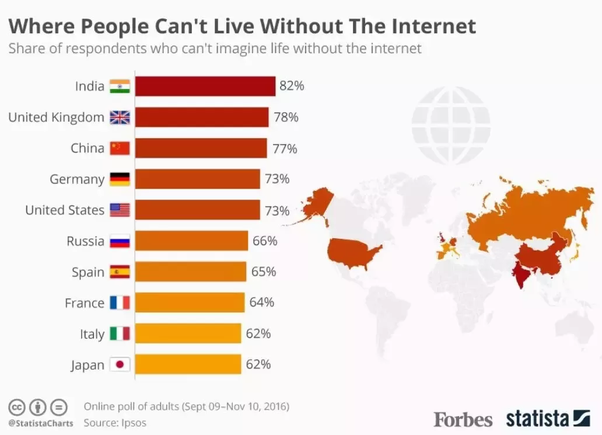
\includegraphics[width=0.8\textwidth]{badsurvey}
            \end{center}
\end{questions}
\end{document}
